% Chapter 4

\chapter[Implementation and on-sky testing]{\setstretch{1}Implementation and on-sky testing} % Main chapter title
\label{chap:implementation}

\epigraph{\setstretch{1}\small\itshape Ever tried. Ever failed. No matter. \\ Try again. Fail again. Fail better.}{S. Beckett}

\section{Key pre-flight procedures}
\subsection{Inertia measurement}
While CAD models allowed to us to estimate the moment of inertia of the payload, this is only an approximation. For testing and for launch, the payload will be different than the model we have: we will either miss some components because they are not yet installed, or have additional components such as the ballasts, the crush pads, or the weights that are used to balance the payload.

We use a simple procedure to estimate the moment of inertia about $\vectors{z}_\gyro$ of the payload while hanging from a crane. For this purpose, we command the CCMG to input a torque to the payload by moving the gimbal at a constant velocity. According to Eq.~\ref{eq:CCMGTorque}, $\ccmgtorque =  20.8\times \dot{\theta}\cos\theta$. According to conservation of angular momentum, the rate of change of the total angular momentum about $\vectors{z}_\gyro$ is $(\inertia\dot{\gyroVec})_\vectors{z} = \ccmgtorque = 20.8\times \dot{\theta}\cos\theta$.

We measure the inertia $\inertia_\vectors{z}$ by averaging measurements of the angular acceleration $\dot{\gyroVec}_\vectors{z}$, divided by the instantaneous input torque, which is numerically more stable than averaging its inverse since the accelerations, expressed in \si{\radian\per\second} are typically very small. A measure of the inertia is then the inverse of this average. By repeating the measurement over multiple accelerations and deceleration cycles, we can also obtain an uncertainty to this estimate.

[PUT HERE A TABLE WITH MEASURED INERTIA AND UNCERTAINTIES]

\subsection{Sensor alignment and calibration}
While the intrinsic noise of our sensors has been characterized in Section~\ref{subsec:gyros}, it is important to test them while mounted to the payload, align their axes to the other reference frames, and study their spectral energy distribution. Mounting the gyroscopes in a 3-dimensional mount on the truss will inevitably lead to alignment errors and the contribution of new vibration frequencies present in the structure and excited by the moving parts on the payload.


\subsubsection{Gyroscope spectral analysis in flight configuration}

The gyroscopes were characterized in quiet laboratory environment that was designed for precision optical interferometry, with special foundations to prevent vibrations being transmitted through the ground. This allowed us to measure the gyroscopes down to their noise levels. However, as soon as we attach the gyroscopes to any structure, the gyroscopes measure their vibration modes. 

\begin{figure}[!h]
\begin{center}
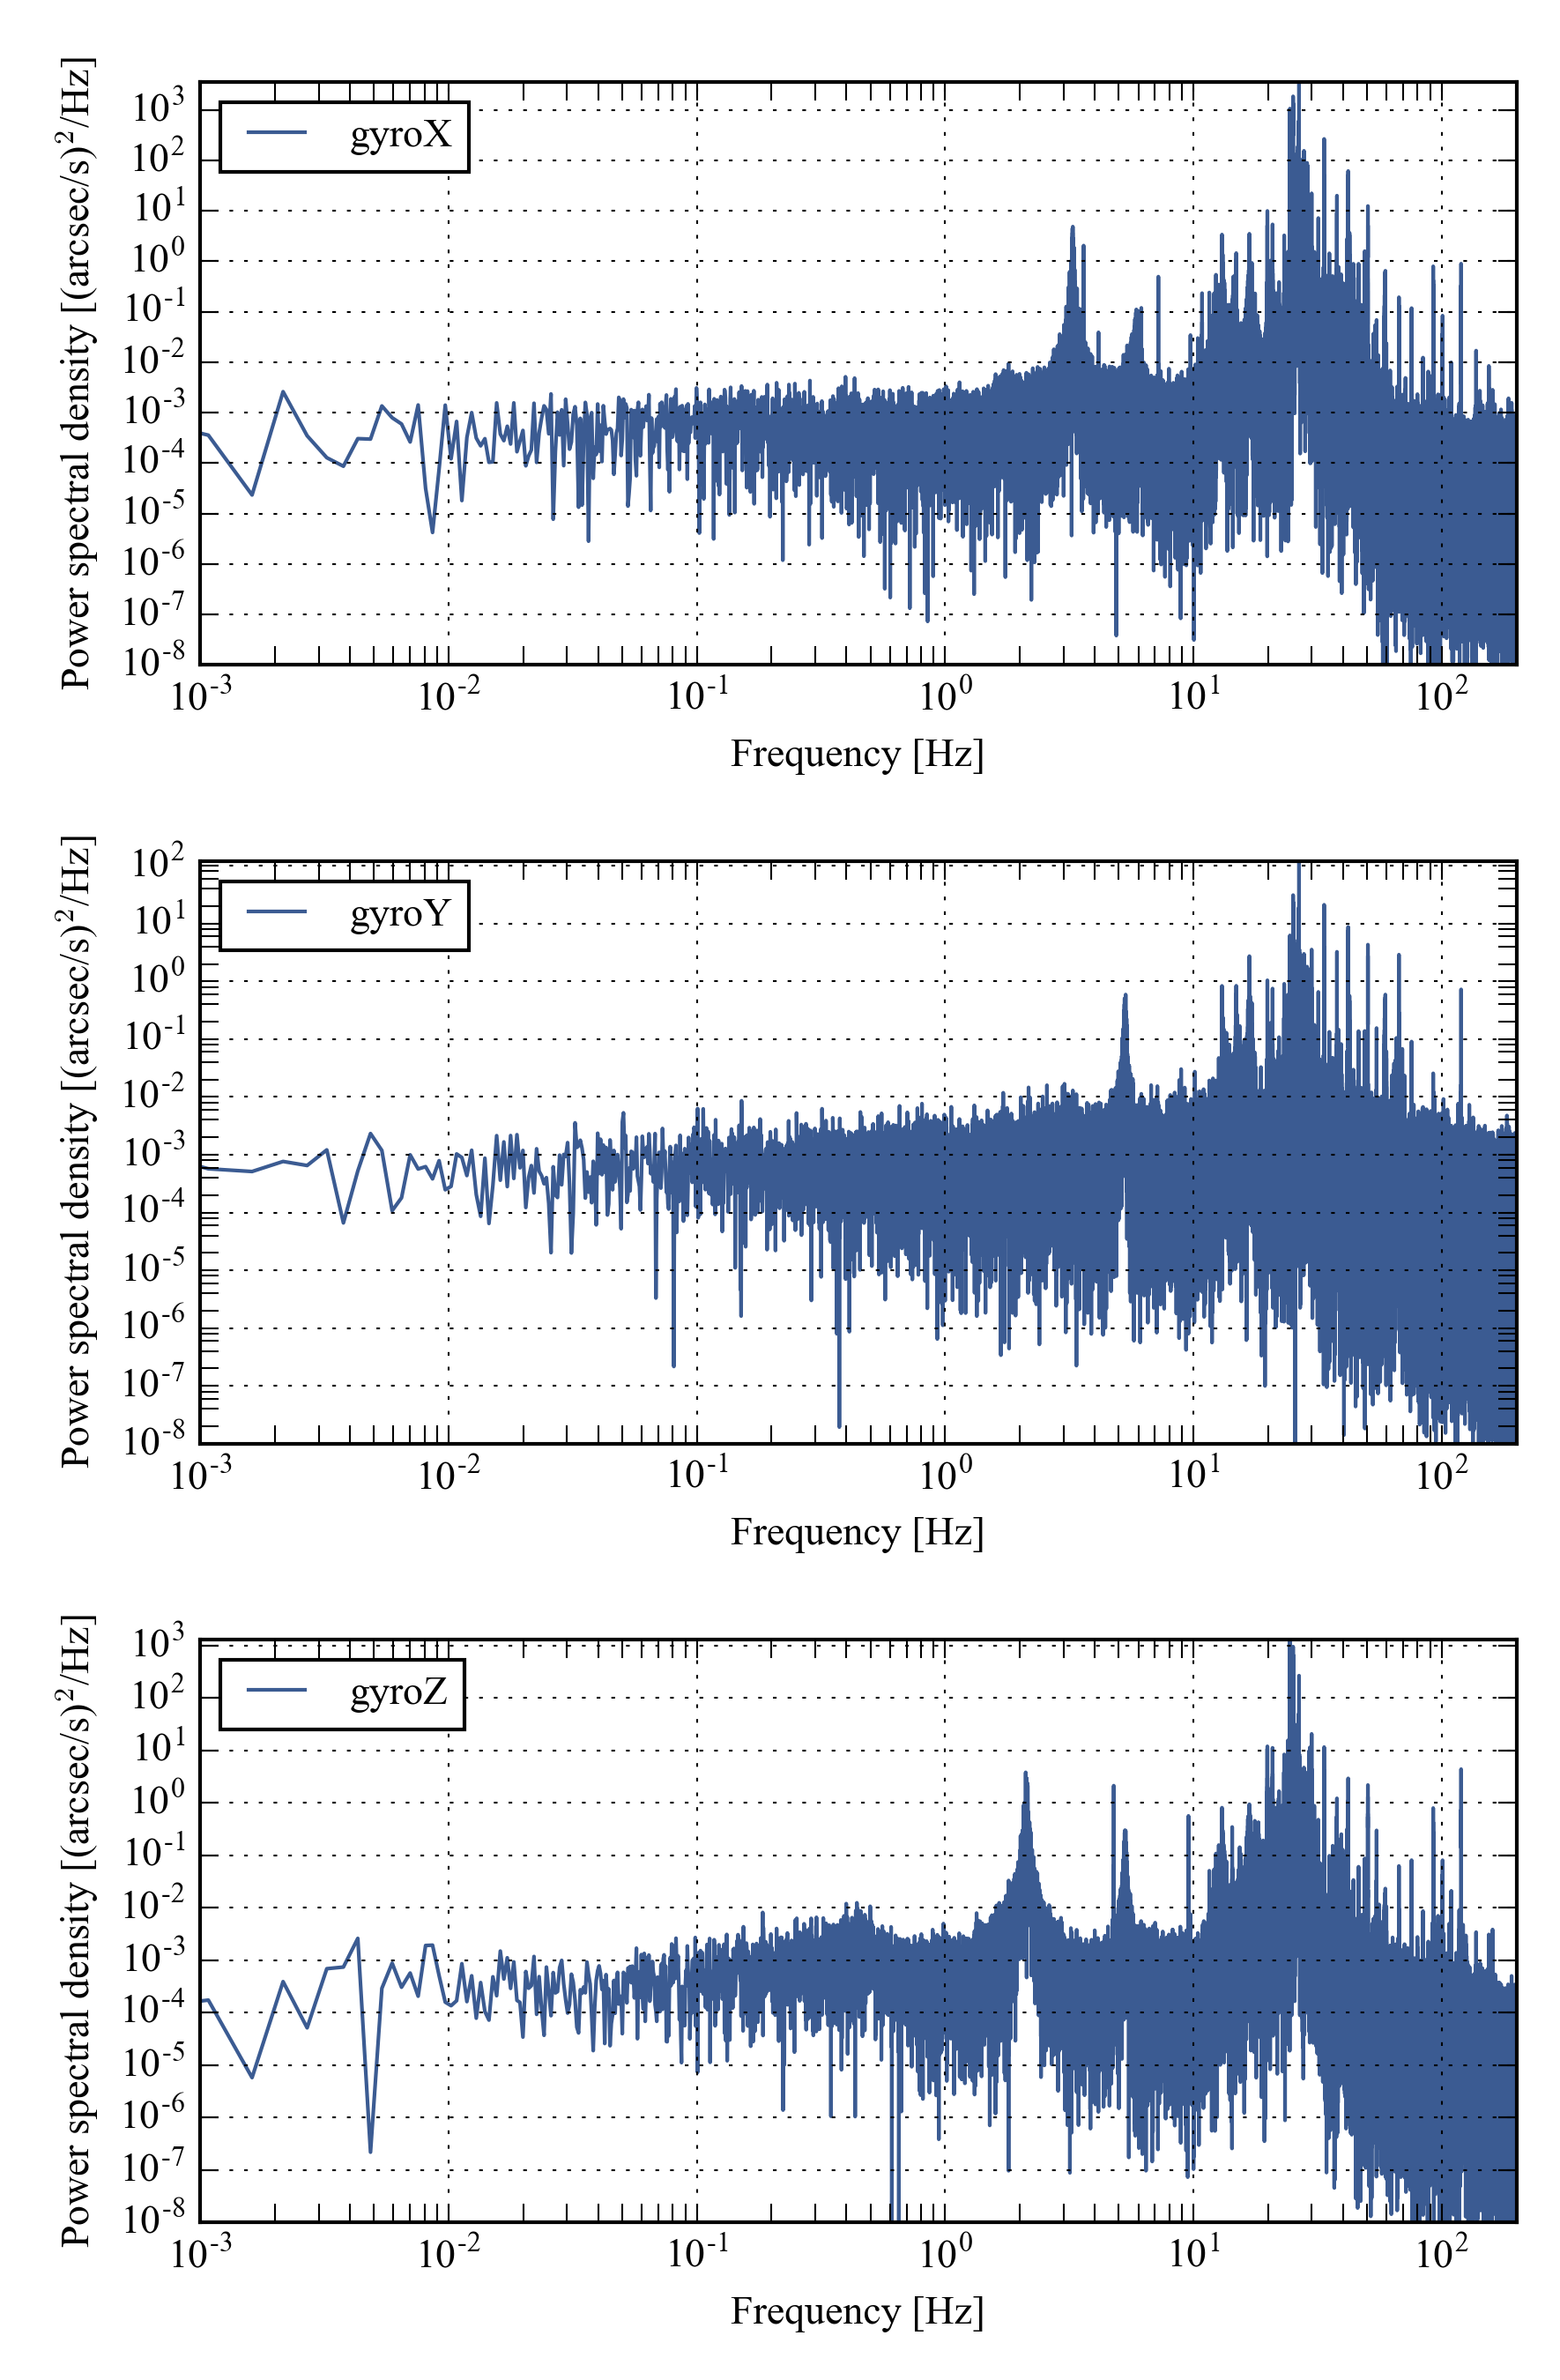
\includegraphics[width=\textwidth]{Figures/multiPSD400.png}
\label{fig:multiPSD400}
\vspace{-0.5cm}
\caption[Gyro PSD with payload on the ground]{Gyro PSD with payload on the ground}
\end{center}
\end{figure}


This is the case for the gyroscope mount. We estimate that, once in the box and attached onto the truss, the gyroscope has $\sim$20 times its natural noise levels. Looking at the power spectral density of the velocity time series (Fig.~\ref{fig:multiPSD400}), almost all of the noise power is contained in three large and sharp peaks, which coincide with the expected carbon fiber structure first resonant modes. These modes are precisely located at 24.49, 25.23 and \SI{26.7}{\hertz} with the mass configuration at which the data was taken, which omits the large siderostat mirrors on each end (Fig.~\ref{fig:multiPSD400_no_loglog_zoom_400}).

The positive conclusion is that the truss has its first resonant frequencies precisely where they were designed to be from CAD modeling, and they are above \SI{20}{\hertz}, which is out of the bandwidth of the attitude control. This noise can then be drastically attenuated either by notch filters (if the frequencies do not shift) or by low-pass filters with a break frequency at a few Hertz. For example at \SI{2.5}{\hertz}, a single-pole low-pass Butterworth filter would attentuate these peaks by \SI{20}{\decibel}, or an attenuation factor of 100. 

Examining the PSD in Fig~\ref{fig:multiPSD400}, we also notice some broad peaks at 3, 5.5, and \SI{2}{\hertz} for the x, y, and z axes respectively. These are attributed to motions of the truss within the gondola about the vibration isolators that were installed to decouple the two mechanical structures. 

\begin{figure}[!h]
\begin{center}
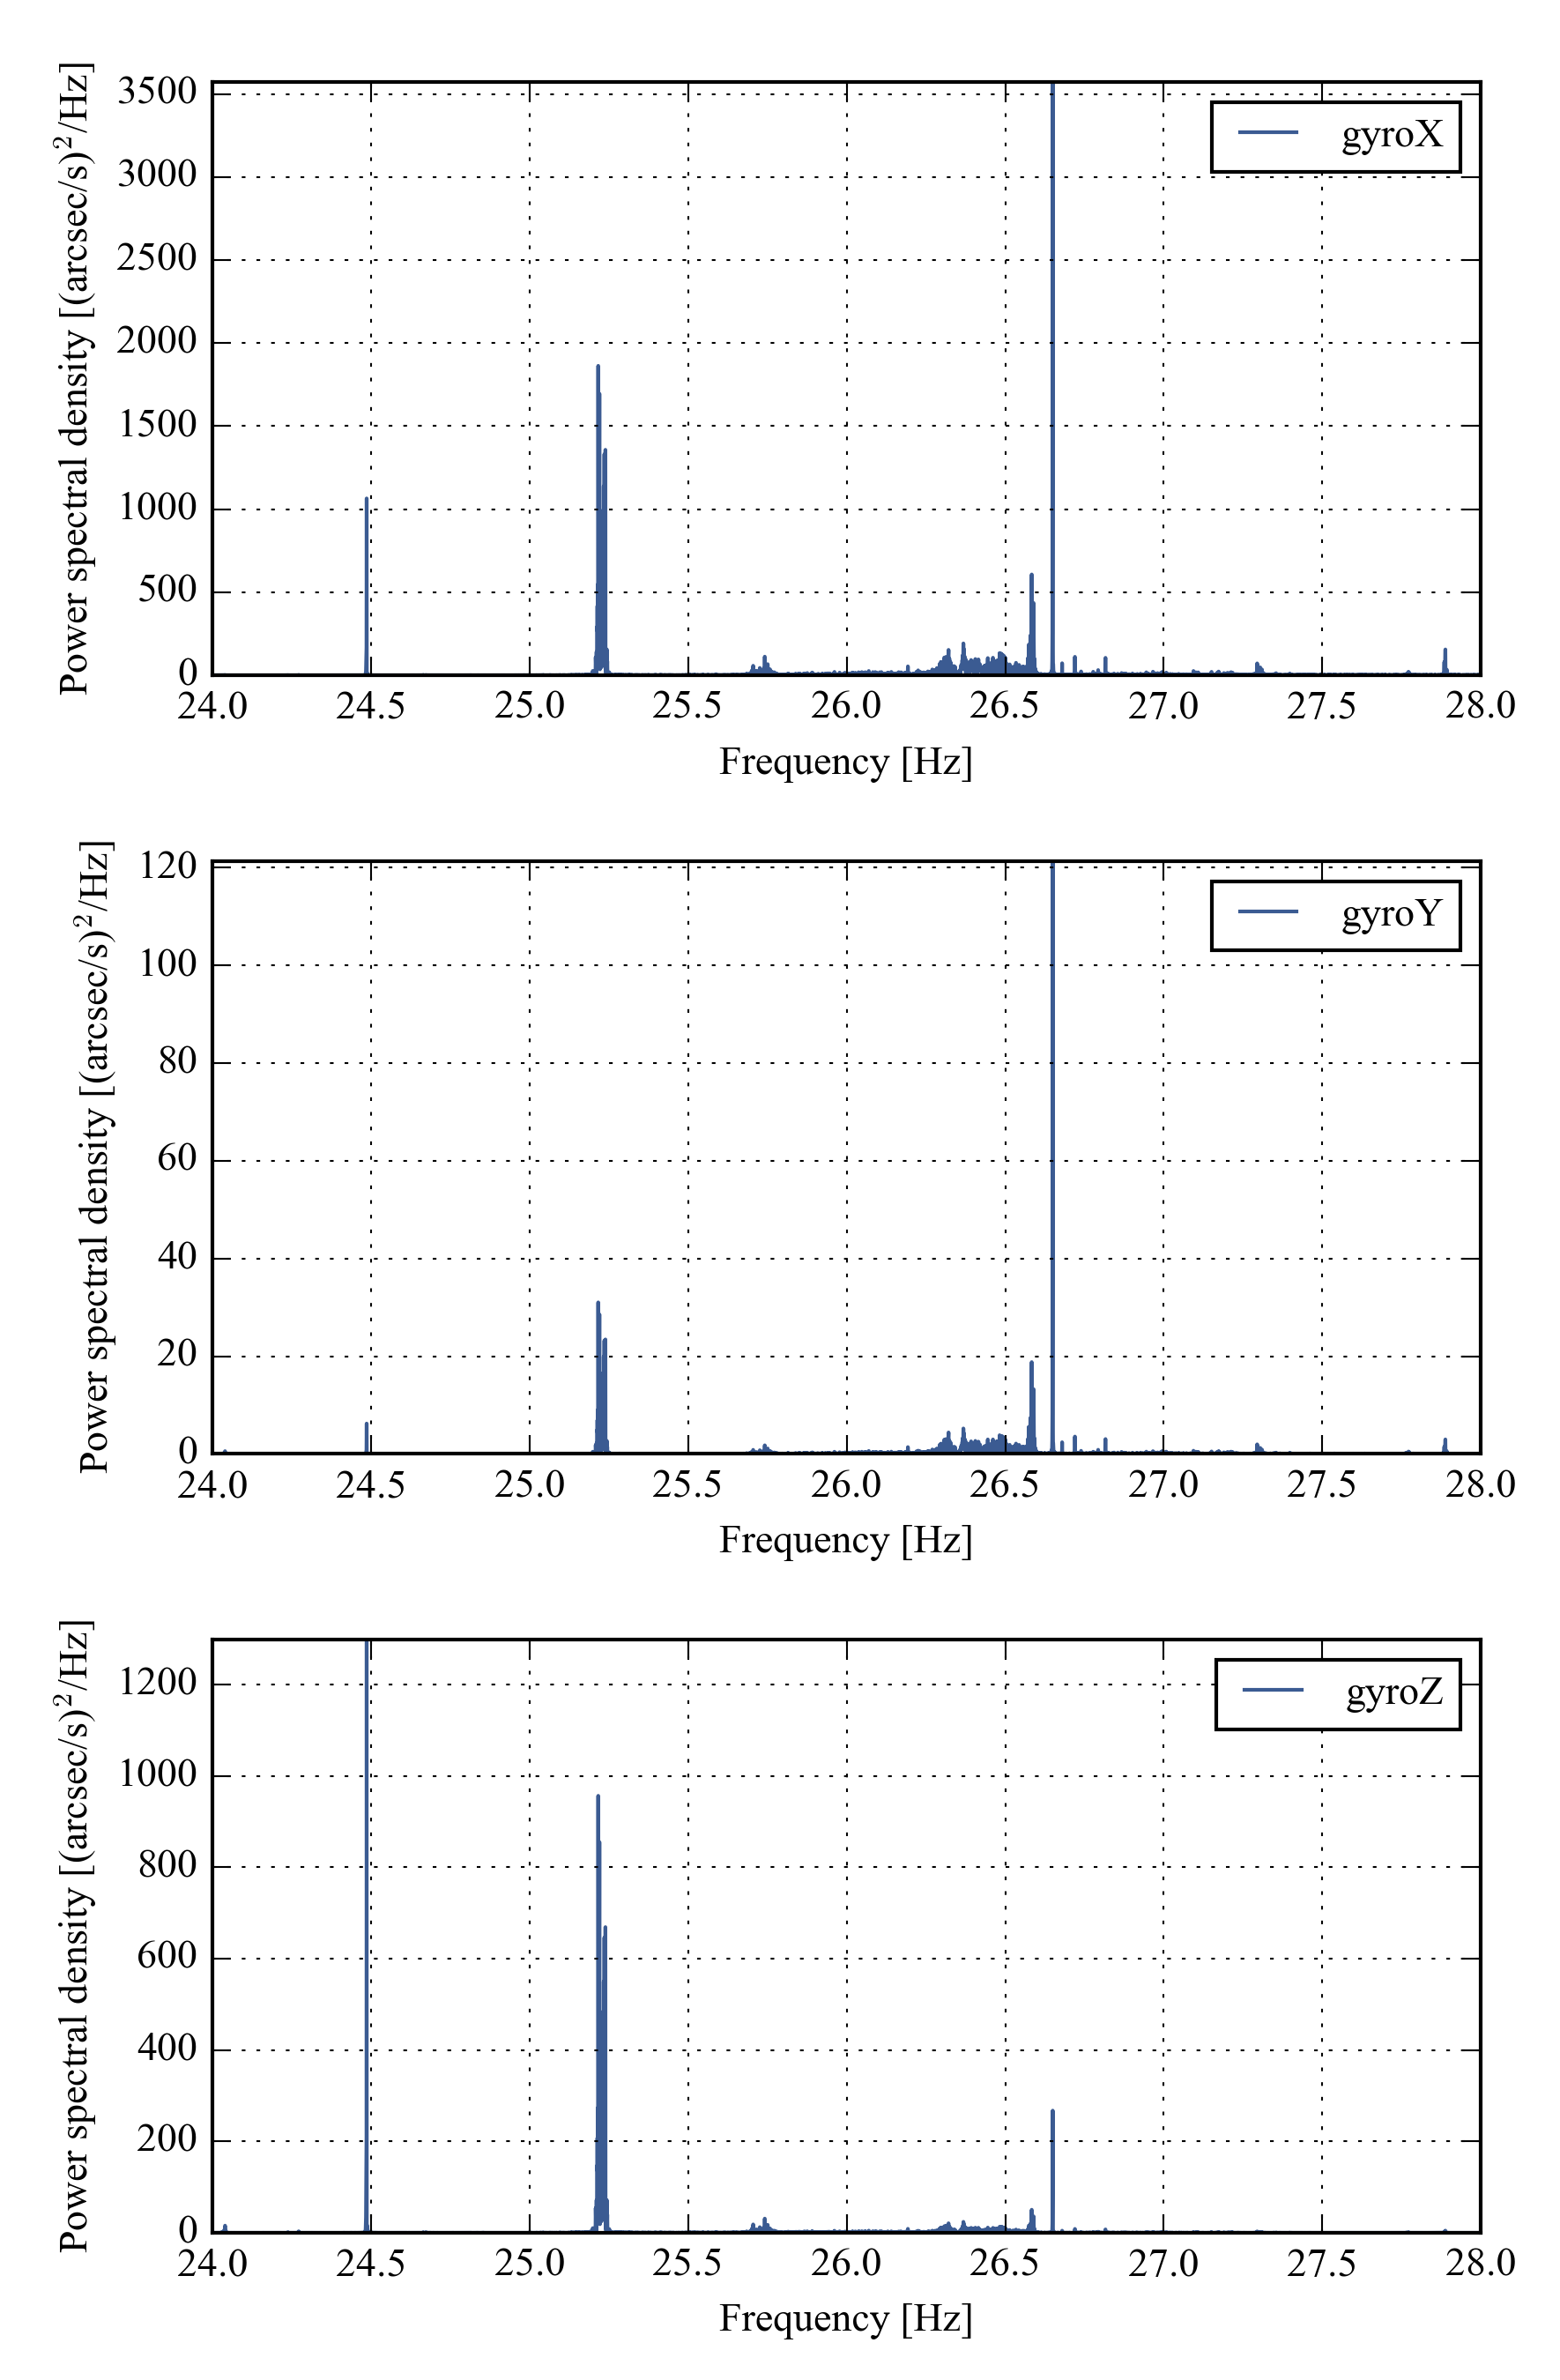
\includegraphics{Figures/multiPSD_no_loglog_zoom_400.png}
\label{fig:multiPSD400_no_loglog_zoom_400}
\vspace{-0.5cm}
\caption[Gyro PSD with payload on the ground - Main peaks]{Gyro PSD with payload on the ground - main peaks.}
\end{center}
\end{figure}



\subsubsection{Orthogonalization of gyroscope mount}
\label{ap:gyroOrth}

An orthogonalization procedure was established to determine the correction matrix to apply to the gyroscope velocity vector to make sure measurement were independent from one another. The procedure involves spinning the 3-axis gyroscope mount on one of the rotation stages that we use for flight (which are used for elevation control). 

The system to solve is:
\begin{equation}
\gyroVec^\textrm{meas} = \begin{bmatrix} M_x & m_{xy} & m_{xz} \\   m_{yx} & M_y &m_{yz} \\  m_{zx} & m_{zy} & M_z \end{bmatrix} \gyroVec^\textrm{true} = M \gyroVec^\textrm{true} 
\end{equation}

The 9 matrix elements can be found by commanding the 3-axis mount to rotate at a known velocity about each axes. Hence, by knowing the vector $\gyroVec^\textrm{true}$ (one component is the commanded velocity and the two others are zero) and measuring the velocities on the three axes, we can determine the matrix element for the column corresponding to the current spin axis. 

The gyroscopes are so sensitive that they measure the rotation of the Earth accurately. This corresponds to a bias in the commanded velocity. To mitigate this issue, we spin the 3-axis mount in two opposite directions. The perceived difference in the velocities corresponds to the Earth velocity about that axis. 

Because of cabling constraints, we are only able to spin the 3-axis mount for small angles. This method works very well when the gyroscope can spin freely and do \SI{360}{\degree} rotations, since a lot of the systematics of the setup will cancel out after multiple revolutions. 

The matrix we obtain suggests typical alignment errors on the order of 0.1-0.3\%, which correspond to angular errors of a few degrees. While the measurements appear to be repeatable, we noticed that the sum of the squares of the velocities was typically 2\% off from its expected value, which we know since it corresponds to the square of the Earth's rotation velocity. Further, this error varies with different orientation of the gyroscope mount. The typical errors that are seen are consistent with a residual misalignment of a few tenths of degrees between the gyroscopes.

This could lead to multiple interpretations. First, it is possible (even likely) that the mount deforms under its own gravity in different ways depending on its orientation. Unfortunately, it is not simple to proceed to this orthogonalization method with the mount in its flight orientation, and would require some ground support equipment (GSE) not available at the moment. 

A second possible interpretation is that the gyroscope internal scale factor is changing. We noted that the temperature of the gyroscopes was increase by about \SI{5}{\degreeCelsius} when they are inside the mount on the thermal isolators. This can potentially change their scale factor (which effectively multiplies the measure velocity) as a result of the fiber optics' length changing slightly. 

The path forward towards orthogonalization of the mount is to use a ROMER metrology arm to measure the relative position of the mount faces to within a few arcminutes. This would allow us to find the components of the matrix $M$ for the mount on the payload in its final flight configuration. It will also allow us to precisely align the mount to the other important reference frames, such as the star camera reference frame and the telescope reference frame.

The scale factor on the $\vectors{z}$ gyroscope can also be precisely determined if the payload if aligned horizontally with precision. Because of the size of the payload, a good lever arm provides an accurate measure of its horizontal position. The gyroscope on the $\vectors{z}$ axis can thus be aligned with the gravity vector precisely, at which point the expected angular velocity is known, and the scale factor correction can be determined.


\subsubsection{Alignment of gyroscope mount to star camera mounts}

Once the gyroscope is orthogonalized, it remains to be properly referenced to the star camera mount. In fact, because those two key elements of the control system are thermally separated, it is possible that they drift between one another. 

For this purpose, we developed a variant to the traditional Kalman filter described in \ref{sec:KalmanFilter}, which instead of estimating the bias, it estimates the rotation matrix between the gyroscope mount and the star camera, as explained in \ref{subsec:enhancedKalman}. 

Running this filter can be done seamlessly, since the number of unknowns is the same as the flight model which estimates bias drifts. 

The problem of using only bias drifts needs some explanation. In the traditional Kalman filter, gyroscope models using only a bias to account for the measurement errors. The bias, which combines linearly with the measured velocity, is adjusted to correct the errors and minimize the covariance of the error.

However, this supposes that the gyroscopes are perfectly orthogonal, with unity scale factor, and the transformation between the measurement sensor (the star camera) reference frame and the gyro reference frame is known perfectly. An error in either of these two components will translate to multiplicative errors on the velocities, which will have a large effect when the velocity dramatically changes (for example, after a slew) and will not be accounted for by a simple bias model. Fig [] illustrates this effect with on-sky data. Eventually, the bias would adjust to be in agreement with the star camera measurements - but it can a while, and during this time, the velocity that we think we are moving at is incorrect. To put this in perspective, a 1\% error on the gyroscope velocity in one axis for a \SI{10}{\degree} slew at \ang{;;400}\si{\per\second} corresponds to a position error of 6 arcminutes, a considerable amount given our pointing requirements.

If this error persists during flight, the poor man's solution is as follows. Instead of tracking the Kalman filter through slew, we slew blindly and reset the estimator after the slew. We reset our starting position with the first solution from the star camera. Since we will be off our target, we will slew again to the desired target, which will be much closer. Each time this needs to be repeated, we minimize the effects of the bias errors.

For our scientific purpose, a 1\% error in the gyroscope scale factor of angular velocity alignment is not a deal breaker, since their main purpose is to maintain sufficient stability to lock onto a guide star with the fine guiding sensor. The fine guiding sensor is by definition in the correct reference frame, since it observes through the optical train. 






\subsection{Star camera}

\subsubsection{Tuning tests}

\renewcommand{\arraystretch}{1.5}
\setlist[itemize,1]{nolistsep,leftmargin=*,labelsep=-\mylen}
\def\labelitemi{--}
\begin{table}[!h]
\scriptsize
\caption[Star camera tests]{Star camera exposure time tests.}
\label{tab:starCameraTests}
\vspace{-0.5cm}
\begin{longtable}{l|P{1.5cm}P{1cm}P{1.5cm}P{1.5cm}P{1.5cm}P{1.5cm}P{1.5cm}P{1.5cm}}													
\toprule																							
{} 	&	  Exposure time (ms)	&	  Number of images in run 	&	  Fitted exposure time (ms)			&	  Number of matching stars 			&	  Fit ra \& dec error (arcsec) 			&	Fit roll error (arcsec)			&	  Processing time (s)			&	  Solution success rate (\%)	\\
\midrule																											
Exp1 	&	250	&	118	&	260	$\pm$	92	&	9.12	$\pm$	1.67	&	1.46	$\pm$	0.43	&	114	$\pm$	40	&	1.48	$\pm$	0.77	&	98	\\
Exp2 	&	125	&	36	&	113	$\pm$	13	&	9.75	$\pm$	1.95	&	1.46	$\pm$	0.39	&	118	$\pm$	32	&	1.05	$\pm$	0.26	&	100	\\
Exp3 	&	62	&	49	&	70	$\pm$	53	&	8.43	$\pm$	1.55	&	1.72	$\pm$	0.64	&	155	$\pm$	66	&	1.01	$\pm$	0.21	&	96	\\
Exp4 	&	62	&	132	&	66	$\pm$	23	&	7.32	$\pm$	1.34	&	1.75	$\pm$	0.65	&	151	$\pm$	55	&	1.22	$\pm$	0.59	&	76	\\
Exp5 	&	31	&	35	&	44	$\pm$	53	&	6.54	$\pm$	0.84	&	2.33	$\pm$	0.79	&	180	$\pm$	65	&	1.19	$\pm$	0.48	&	37	\\
\bottomrule
\end{longtable}																							
\end{table}																							

\begin{landscape}
\begin{figure}[!ht]
	\centering
	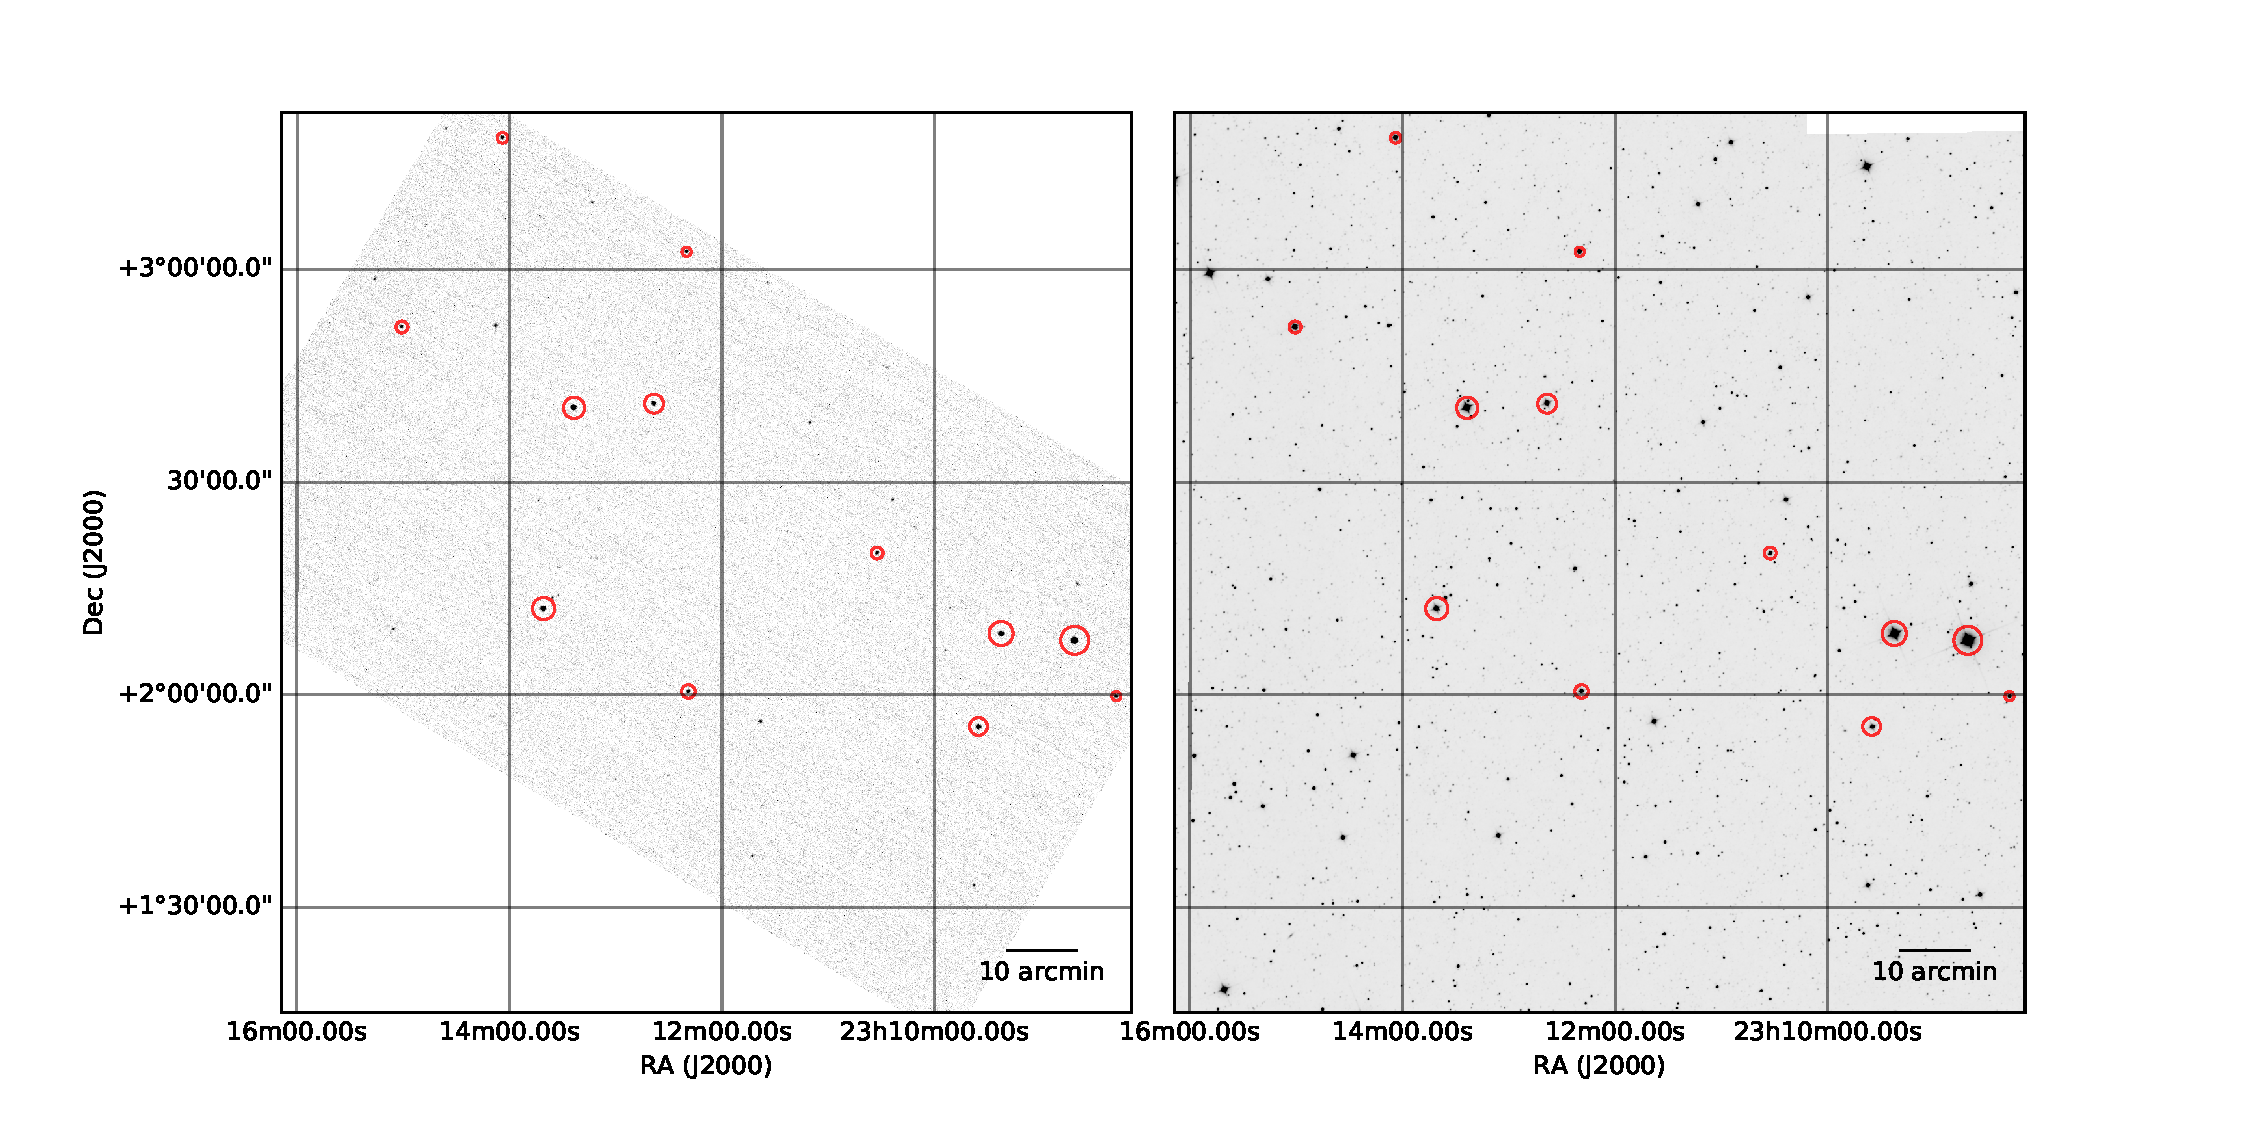
\includegraphics[width=1.5\textwidth]{Figures/starcam_images.pdf}
	\caption[Star camera example WISE]{\textit{Left}: Example of a background-subtracted star camera image with identified $>5\sigma$ sources circled in red. The orientation of the image on the celestial sphere is the one provided by BETTII's embedded star camera solver. This image corresponds to a field in the Scorpius constellation. \textit{Right}: WISE \SI{3.4}{\um} mosaic from the online archive, centered on the same location. This image is composed of 9 individual WISE images that we patched into a mosaic using the \textit{Montage}[CITE] software package.}
	\label{fig:starcamexample}
    \end{figure}
\end{landscape}
\begin{landscape}
\begin{figure}[!ht]
	\centering
	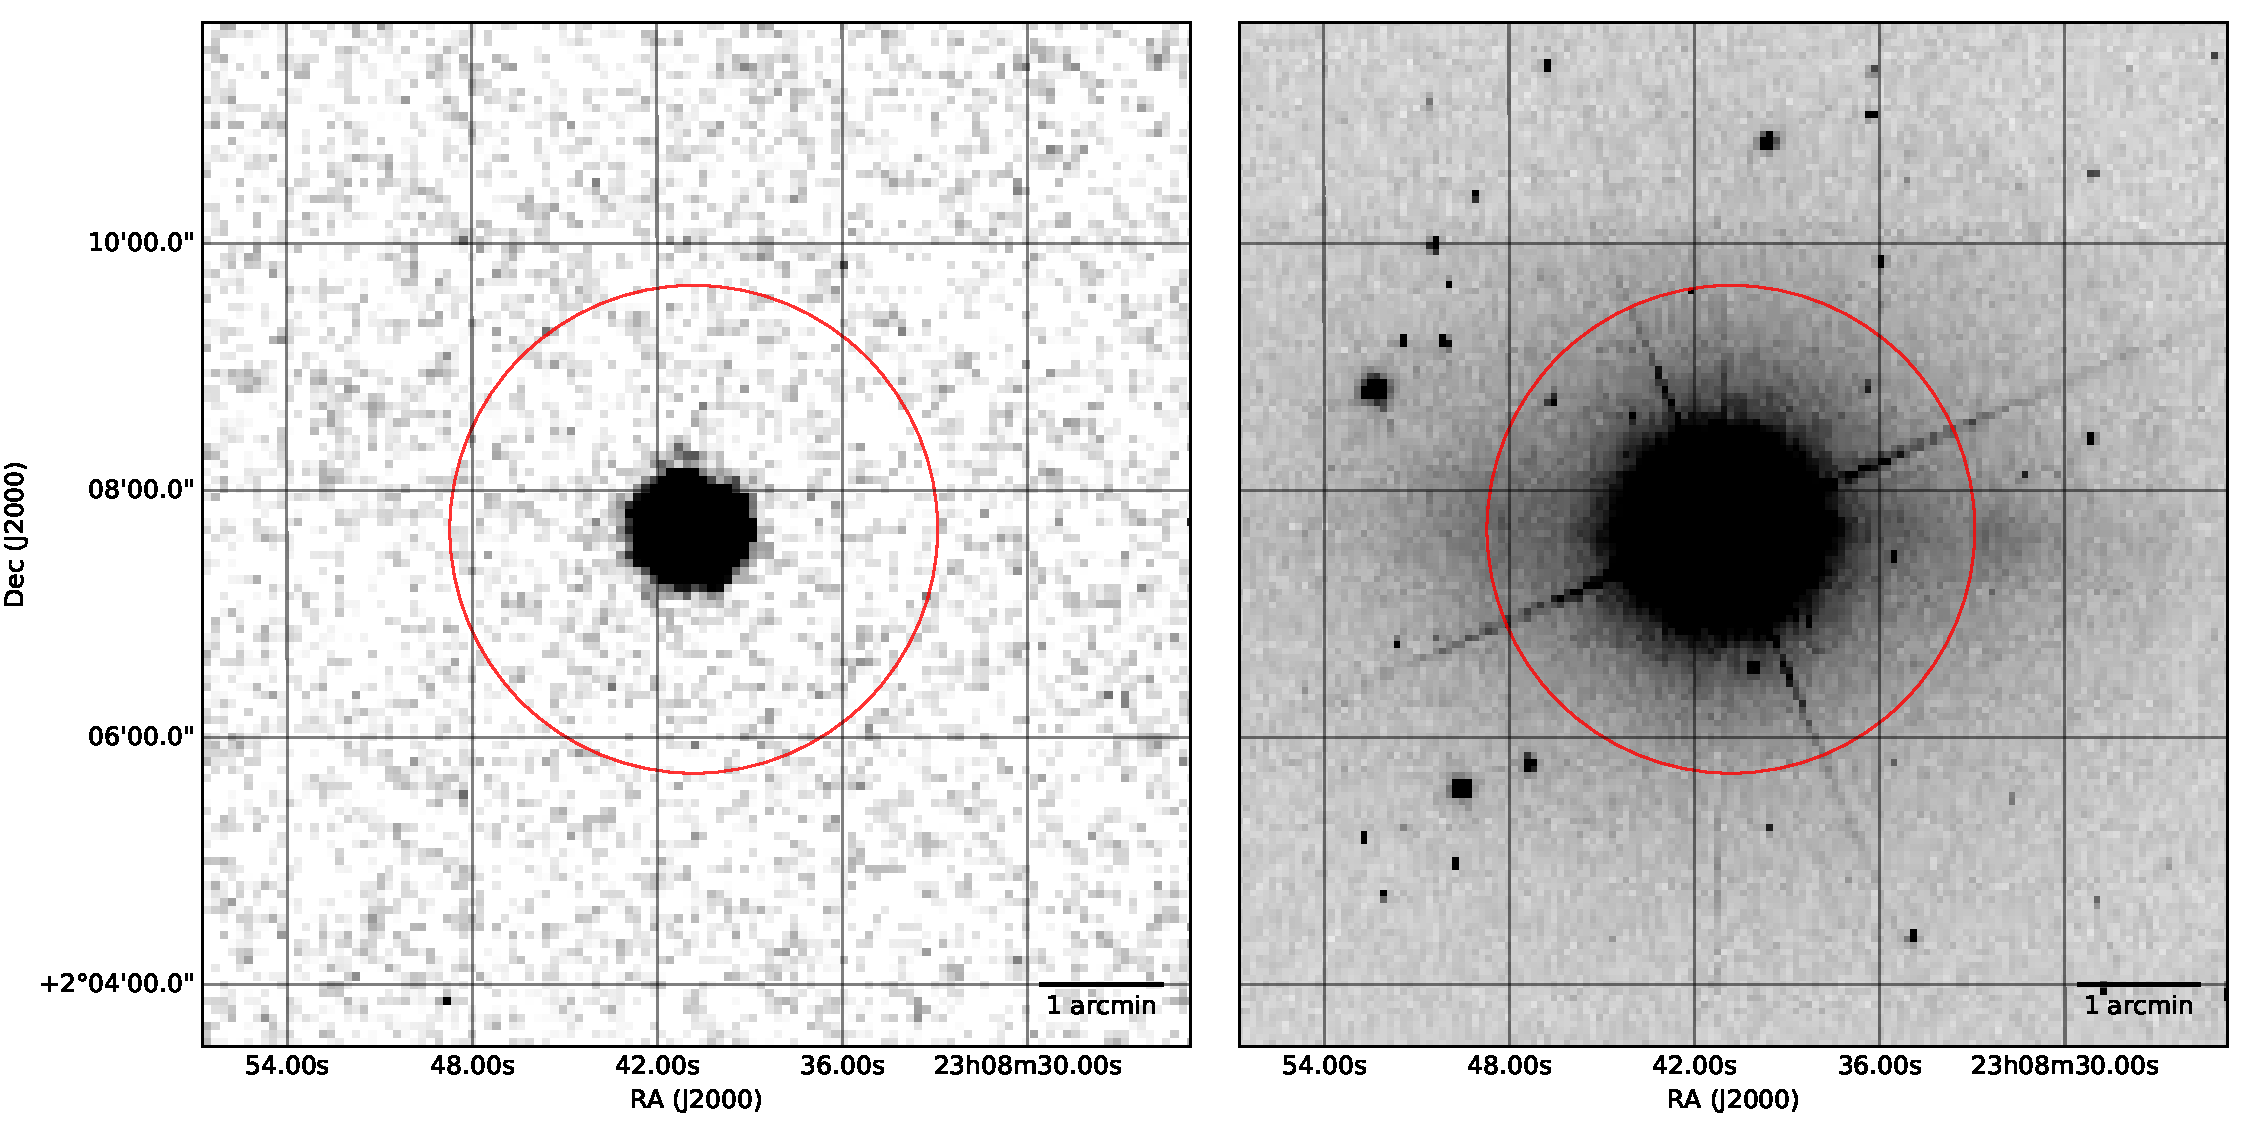
\includegraphics[width=1.5\textwidth]{Figures/starcam_SDSSr_zoom.pdf}
	\caption[Star camera individual star]{\textit{Left}: Snapshot of a bright star seen within the background-subtracted star camera frame. \textit{Right}: Snapshot taken at the same location from the WISE \SI{3.4}{\um} archive.}
	\label{fig:starcamzoom}
    \end{figure}
\end{landscape}

Discuss about tuning, catalog, filters, etc

Table with the star camera parameters

Show mean deviation of star camera image with optimized parameters;
show time, statistics, etc.

\subsubsection{Final parameters}

\section{Test setups and limitations}
\subsection{Talk about the way we test in the high bay, etc}
\subsection{List of test setups: gyro only, gyro+star camera, gyro+star camera+tip/tilts with CCD cameras, gyro+star camera with H1RG;}
\subsection{Explain the communication/data recording approach}

\subsection{Autofocus algorithm and performance}

\section{Estimator implementation}
\subsection{Gyro attitude estimator}
\documentclass{standalone}
\usepackage{tikz}
\usetikzlibrary{shapes,arrows}

\begin{document}
\tikzstyle{block} = [draw, fill=black!20, rectangle, 
    minimum height=3em, minimum width=6em,align=center]
\tikzstyle{input} = [node distance=1cm]
\tikzstyle{output} = [node distance=1cm]
\newpage
\begin{tikzpicture}[auto, >=latex',scale=0.8, every node/.style={transform shape}]
\linespread{1}


% Inputs
\node [input,name=measuredVelocity,shift={(2cm,0cm)}] {$\gyroVec^{\textrm{meas}}_k$};
\node [input,above of=measuredVelocity,name=bias] {$\EstBias_{k|k-N}$};
\node [input,above of=bias,name=attitude,node distance=1cm] {$\EstAttitude_{k-1|k-N}$};
\node [input,above of=measuredVelocity,name=covariance,node distance=3cm] {$\noiseCovMat_k$};
\node [input,below of=measuredVelocity,name=propagation matrices,node distance=4cm] {$\A_{k-1},\B_{k-1},\C_{k-1}$};

% line break
\node [input,name=line break left,above of=covariance,node distance=2cm] {};
\node [input,name=line break left2,below of=line break left,node distance=0.5cm,right] {\large \textbf{Kalman Filter: Prediction}};
\node [input,name=line break right,right of=line break left,node distance=15cm] {\large { }};
\draw[dashed] ([xshift=-1cm]line break left.north west) -- (line break right.north east);


% blocks
\node [block, right of=measuredVelocity,node distance=3cm] (estimate velocity) {Estimate \\ Velocity};
\node [block, right of=estimate velocity,node distance=4cm] (predict attitude) {Predict \\ Attitude};
\node [block, below of=predict attitude,node distance=2cm] (state transition) {State \\ transition};
\node [block, right of=state transition,node distance=4cm] (estimate covariance) {Estimate \\ covariance};
\node [block, below of=estimate covariance,node distance=2cm] (update propagation matrices) {Propagate \\ matrices};

% outputs
\node [output,right of=predict attitude,node distance=3cm,name=estattitude]{};
\node [output,right of=estimate covariance,node distance=3cm,name=estcovariance]{};
\node [output,right of=update propagation matrices,node distance=3cm,name=propmat]{};

% arrows
\draw[->] (bias.east) -| (estimate velocity.north);
\draw[->] (measuredVelocity.east) -- (estimate velocity.west);

\node[name=mid,right of=estimate velocity,node distance=2cm,draw,fill,minimum size=3pt,circle]{};
\node[above] at (mid){$\EstGyroVec_{k|k-N}$};
\draw[->] (estimate velocity.east) -- (mid) -- (predict attitude.west);
\draw[->] (attitude.east) -| (predict attitude.north);
\draw[->] (mid) |- (state transition.west) ;
\node[name=mid,right of=state transition,node distance=2cm,draw,fill,minimum size=3pt,circle]{};
\node[above] at (mid){$\StateTransitionMat_k$};
\draw[->] (state transition.east) -- (mid) -- (estimate covariance.west) ;
\node[name=mid2,below of=mid,node distance=1cm,outer sep=0cm,inner sep=0cm]{};
\draw[-] (mid) --  (mid2.north) ;
\draw[->] (mid2.north) -|  (update propagation matrices.north) ;

\node[name=mid,right of=estimate covariance,node distance=3cm]{};
\node[above] at (mid){$\stateCovMat_{k|k-N}$};
\draw[->] (estimate covariance.east) -- (estcovariance) ;
\draw[->] (covariance.east) -| (estimate covariance.north) ;

\node[name=mid,right of=predict attitude,node distance=3cm]{};
\node[above] at (mid){$\EstAttitude_{k|k-N}$};
\draw[->] (predict attitude.east) -- (mid);

\draw[->] (propagation matrices.east) -- (update propagation matrices.west);
\draw[->] (update propagation matrices.east) -- (propmat);
\node[name=mid,right of=update propagation matrices,node distance=3cm]{};
\node[above] at (mid){$\A_{k},\B_{k},\C_{k}$};


% Kalman Update
% line break
\node [input,name=line break left,below of=propagation matrices,node distance=1.5cm] {};
\node [input,name=line break left2,below of=line break left,node distance=0.5cm,right] {\large \textbf{Kalman Filter: Update}};
\node [input,name=line break right,right of=line break left,node distance=15cm] {\large { }};
\draw[dashed] ([xshift=-1cm]line break left.north west) -- (line break right.north east);

% Inputs
\node [input,name=measured attitude,below of=line break left,node distance=3cm] {$\Attitude^\textrm{meas}_{\starcam}$};
\node [input,name=final matrices,above of=measured attitude,node distance=1cm] {$\A_{k},\B_{k},\C_{k}$};
\node [input,name=covmat,below of=measured attitude,node distance=6cm] {$\stateCovMat_{k|k-N}$};
\node [input,name=meascovmat,below of=measured attitude,node distance=2cm] {$\measCovMat_{k}$};

% blocks
\node [block, right of=measured attitude,node distance=3cm] (propagate attitude) {Rotate \& \\ Propagate};
\node [block, below of=propagate attitude,node distance=2cm] (innovation) {Innovation};
\node [block, below of=innovation,node distance=2cm] (innovation covariance) {Innovation \\ covariance};
\node [block, below of=innovation covariance,node distance=2cm] (kalman gain) {Kalman \\ gain};
\node [block, right of=kalman gain,node distance=4cm] (calculate error) {Calculate \\ error};
\node [block, right of=calculate error,node distance=4cm] (update bias) {Update \\ bias};
\node [block, below of=update bias,node distance=2cm] (update attitude) {Update \\ attitude};
\node [block, above of=update bias,shift={(3cm,1cm)}] (update velocity) {Update \\ velocity};
\node [block, below of=update attitude,node distance=2cm] (update covariance) {Update \\ covariance};

% arrows
\draw[->] (measured attitude) -- (propagate attitude);
\draw[->] (final matrices) -| (propagate attitude);
\draw[->] (propagate attitude.south) -- (innovation.north);
\draw[->] (innovation covariance.south) -| (kalman gain.north);
\draw[->] (covmat.east) -- (kalman gain.west);
\draw[->] (covmat.north) |- (innovation covariance.west);
\draw[->] (meascovmat.east) -- (innovation.west);
\draw[->] (covmat.south) |- (update covariance.190);

% intermediary nodes
\node[name=mid,right of=kalman gain,node distance=2cm,draw,fill,minimum size=3pt,circle]{};
\node[above] at (mid){$\KalmanGain_{k}$};
\draw[->] (kalman gain.east) -- (mid) -- (calculate error.west);
\draw[->] (mid) |- (update covariance.165);

\node[name=mid,below of=propagate attitude,node distance=1cm]{};
\node[left] at (mid){$\Attitude^{\textrm{meas}}_{k}$};


\node[name=mid,below of=innovation,node distance=1cm,draw,fill,minimum size=3pt,circle]{};
\node[left] at (mid){$\zMeasurement_{k}$};
\draw[->] (mid) -| (calculate error.north);
\draw[->] (innovation.south) -- (mid) -- (innovation covariance.north);

\node[name=mid,below of=innovation covariance,node distance=1cm]{};
\node[left] at (mid){$\measErrCovMat_{k}$};


\node[name=mid,right of=calculate error,node distance=2cm,draw,fill,minimum size=3pt,circle]{};
\node[above] at (mid){$\ErrorState_{k|k}$};
\draw[->] (calculate error.east) -- (mid) -- (update bias.west);

\node [input,name=bias estimate,above of=mid,shift={(1cm,0cm)}] {$\EstBias_{k|k-N}$};
\draw[->] (bias estimate) -| (update bias.north);

\node [input,name=attitude estimate,below of=bias estimate,node distance=2cm] {$\EstAttitude_{k|k-N}$};
\draw[->] (attitude estimate) -| (update attitude.north);


\node [input,name=velocity estimate,above of=bias estimate,node distance=2cm] {$\EstGyroVec_{k|k-N}$};
\draw[->] (velocity estimate) -| (update velocity.north);
\draw[->] (mid) |- (update attitude.west);

\node [output,name=velocity,right of=update velocity,node distance=2cm]{}; \node [output,right of=update velocity,node distance=2cm,above] {$\EstGyroVec_{k|k}$};
\draw[->] (update velocity.east) -- (velocity);

% outputs
\node [output,name=mid,right of=update bias,node distance=3cm,draw,fill,minimum size=3pt,circle] {};
\draw[->] (update bias.east) -- (mid);
\draw[->] (mid) -- (update velocity.south);
\node [output,name=bias,right of=mid,node distance=2cm] {};
\node [output,right of=mid,node distance=2cm,above] {$\EstBias_{k|k}$};
\draw[->] (mid) -- (bias.west);
\node [output,name=attitude,right of=update attitude,node distance=2cm] {};
\node [output,right of=update attitude,node distance=2cm,above] {$\EstAttitude_{k|k}$};
\draw[->] (update attitude) -- (attitude);

\node [output,name=covariances,right of=update covariance,node distance=2cm] {};
\node [output,right of=update covariance,node distance=2cm,above] {$\stateCovMat_{k|k}$};
\draw[->] (update covariance) -- (covariances);

\end{tikzpicture}
\end{document}

\subsubsection{Testing the Kalman filter software with simulated data}
\subsubsection{Test results when sitting on the ground}
\subsection{Telescope attitude estimator}
Link to cross-elevation
\subsection{Phase estimator [is that Arnab’s realm?]}

\section{Operating modes}
\subsection{Track mode}
Gain tuning
Show wheel angle for long time
\subsection{Slew mode}
\subsection{Acquire mode [this one is contingent on the telescopes working, and is not perfectly representative when only using one single side of the payload]}

\section{Pointing tests and performance results}
\subsection{Gondola pointing stability}
\subsubsection{In the high bay}

\begin{figure}[!ht]
\begin{center}
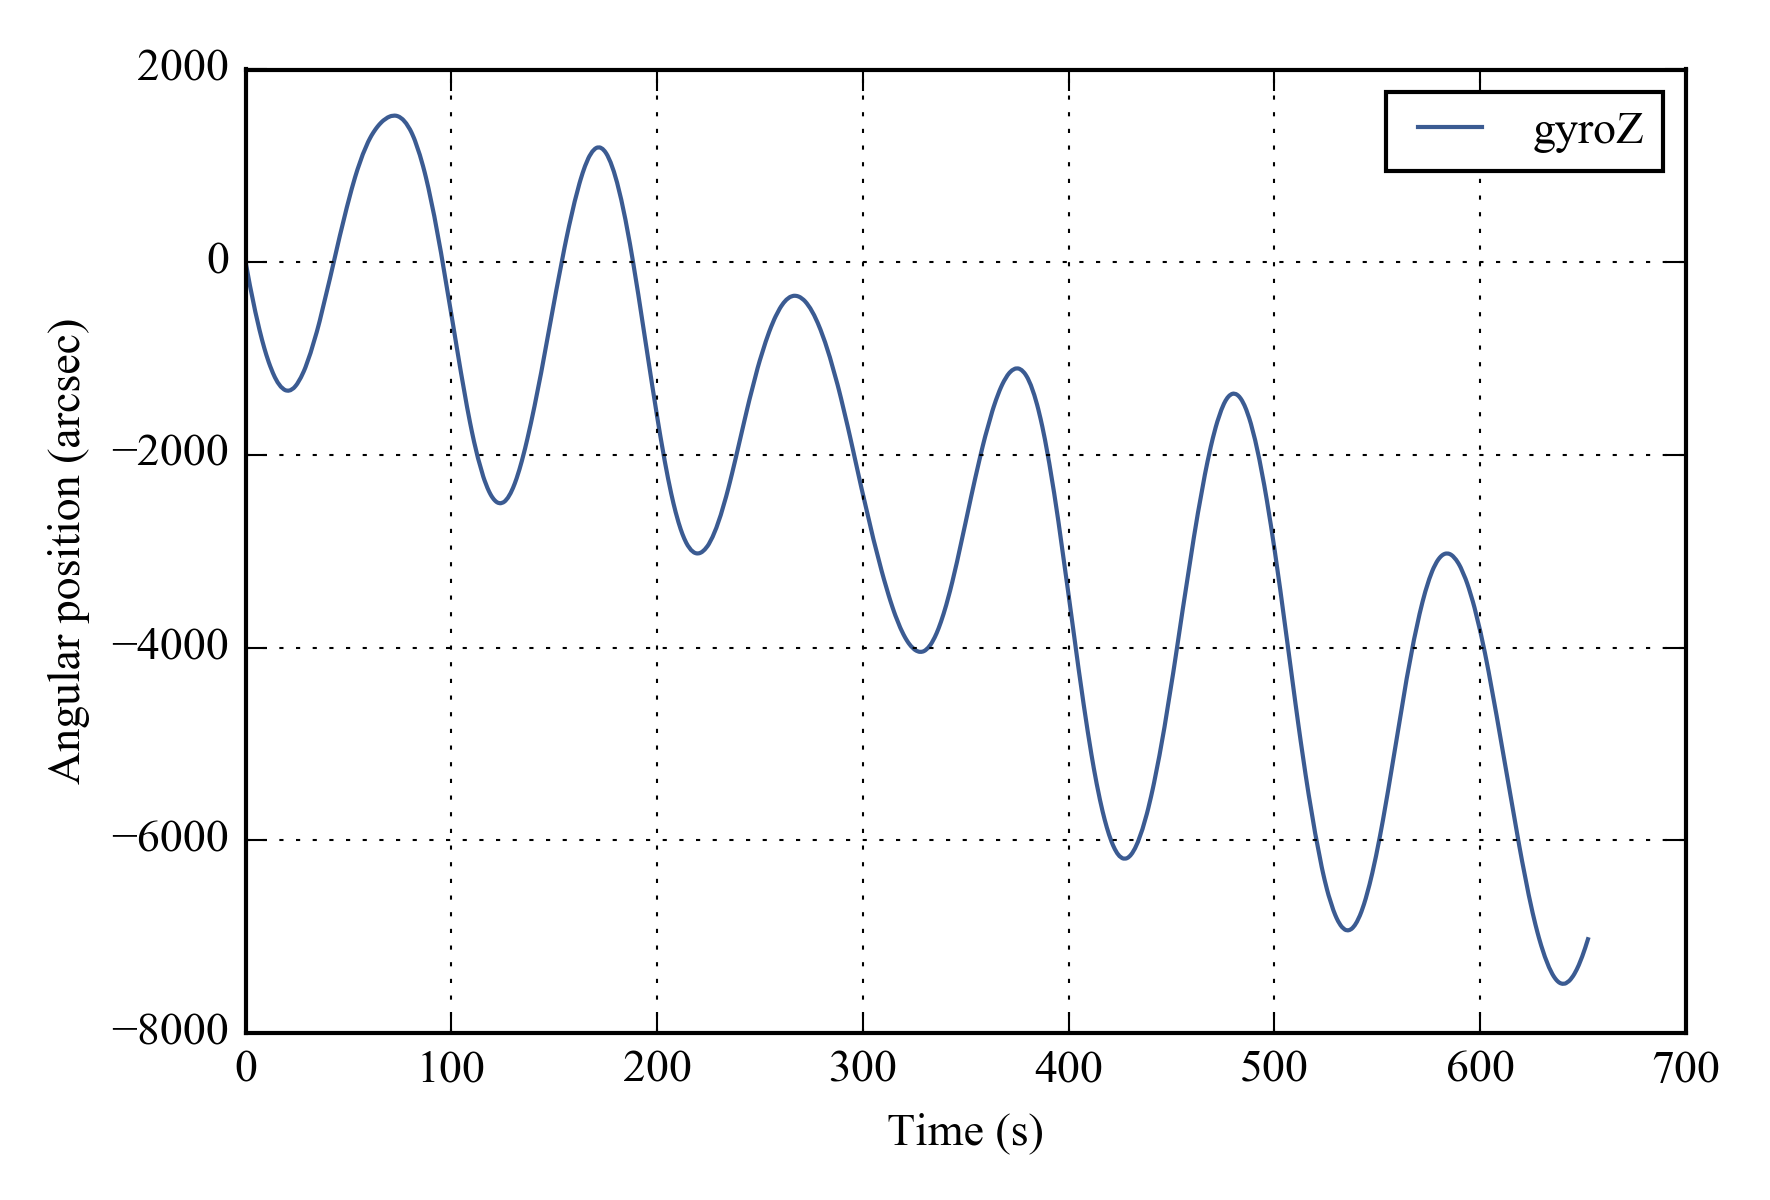
\includegraphics{Figures/integral_lifted_gyroZ.png}
\label{fig:intgralgyroZ400}
\vspace{-0.5cm}
\caption[Integrated gyro time series while hanging]{Integrated gyro time series while hanging and no motor on.}
\end{center}
\end{figure}
\begin{figure}[!h]
\begin{center}
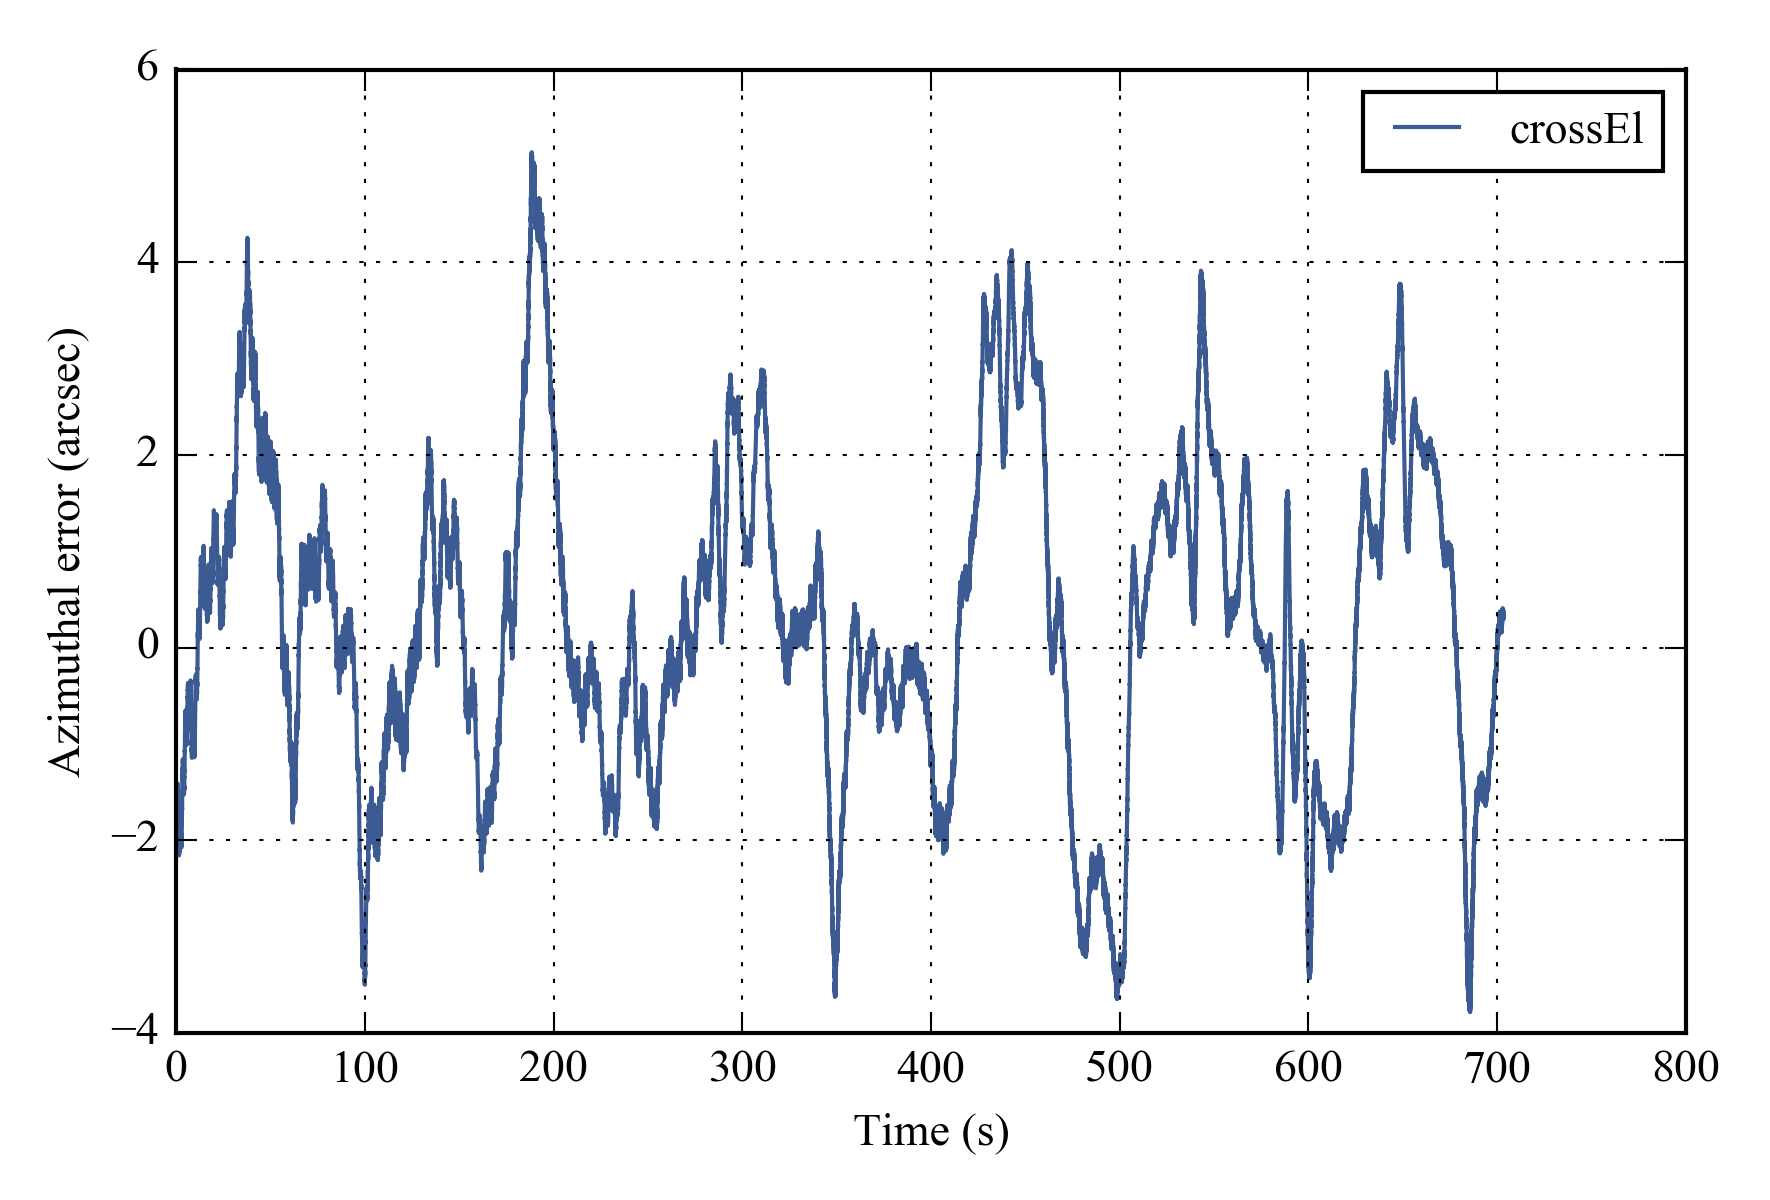
\includegraphics[width=\textwidth]{Figures/simplePlot_crossEl.png}
\label{fig:crossEl400}
\vspace{-0.5cm}
\caption[Cross-elevation with control loop on]{Cross-elevation with control loop on (gyroscopes only).}
\end{center}
\end{figure}




\begin{figure}[!h]
\begin{center}
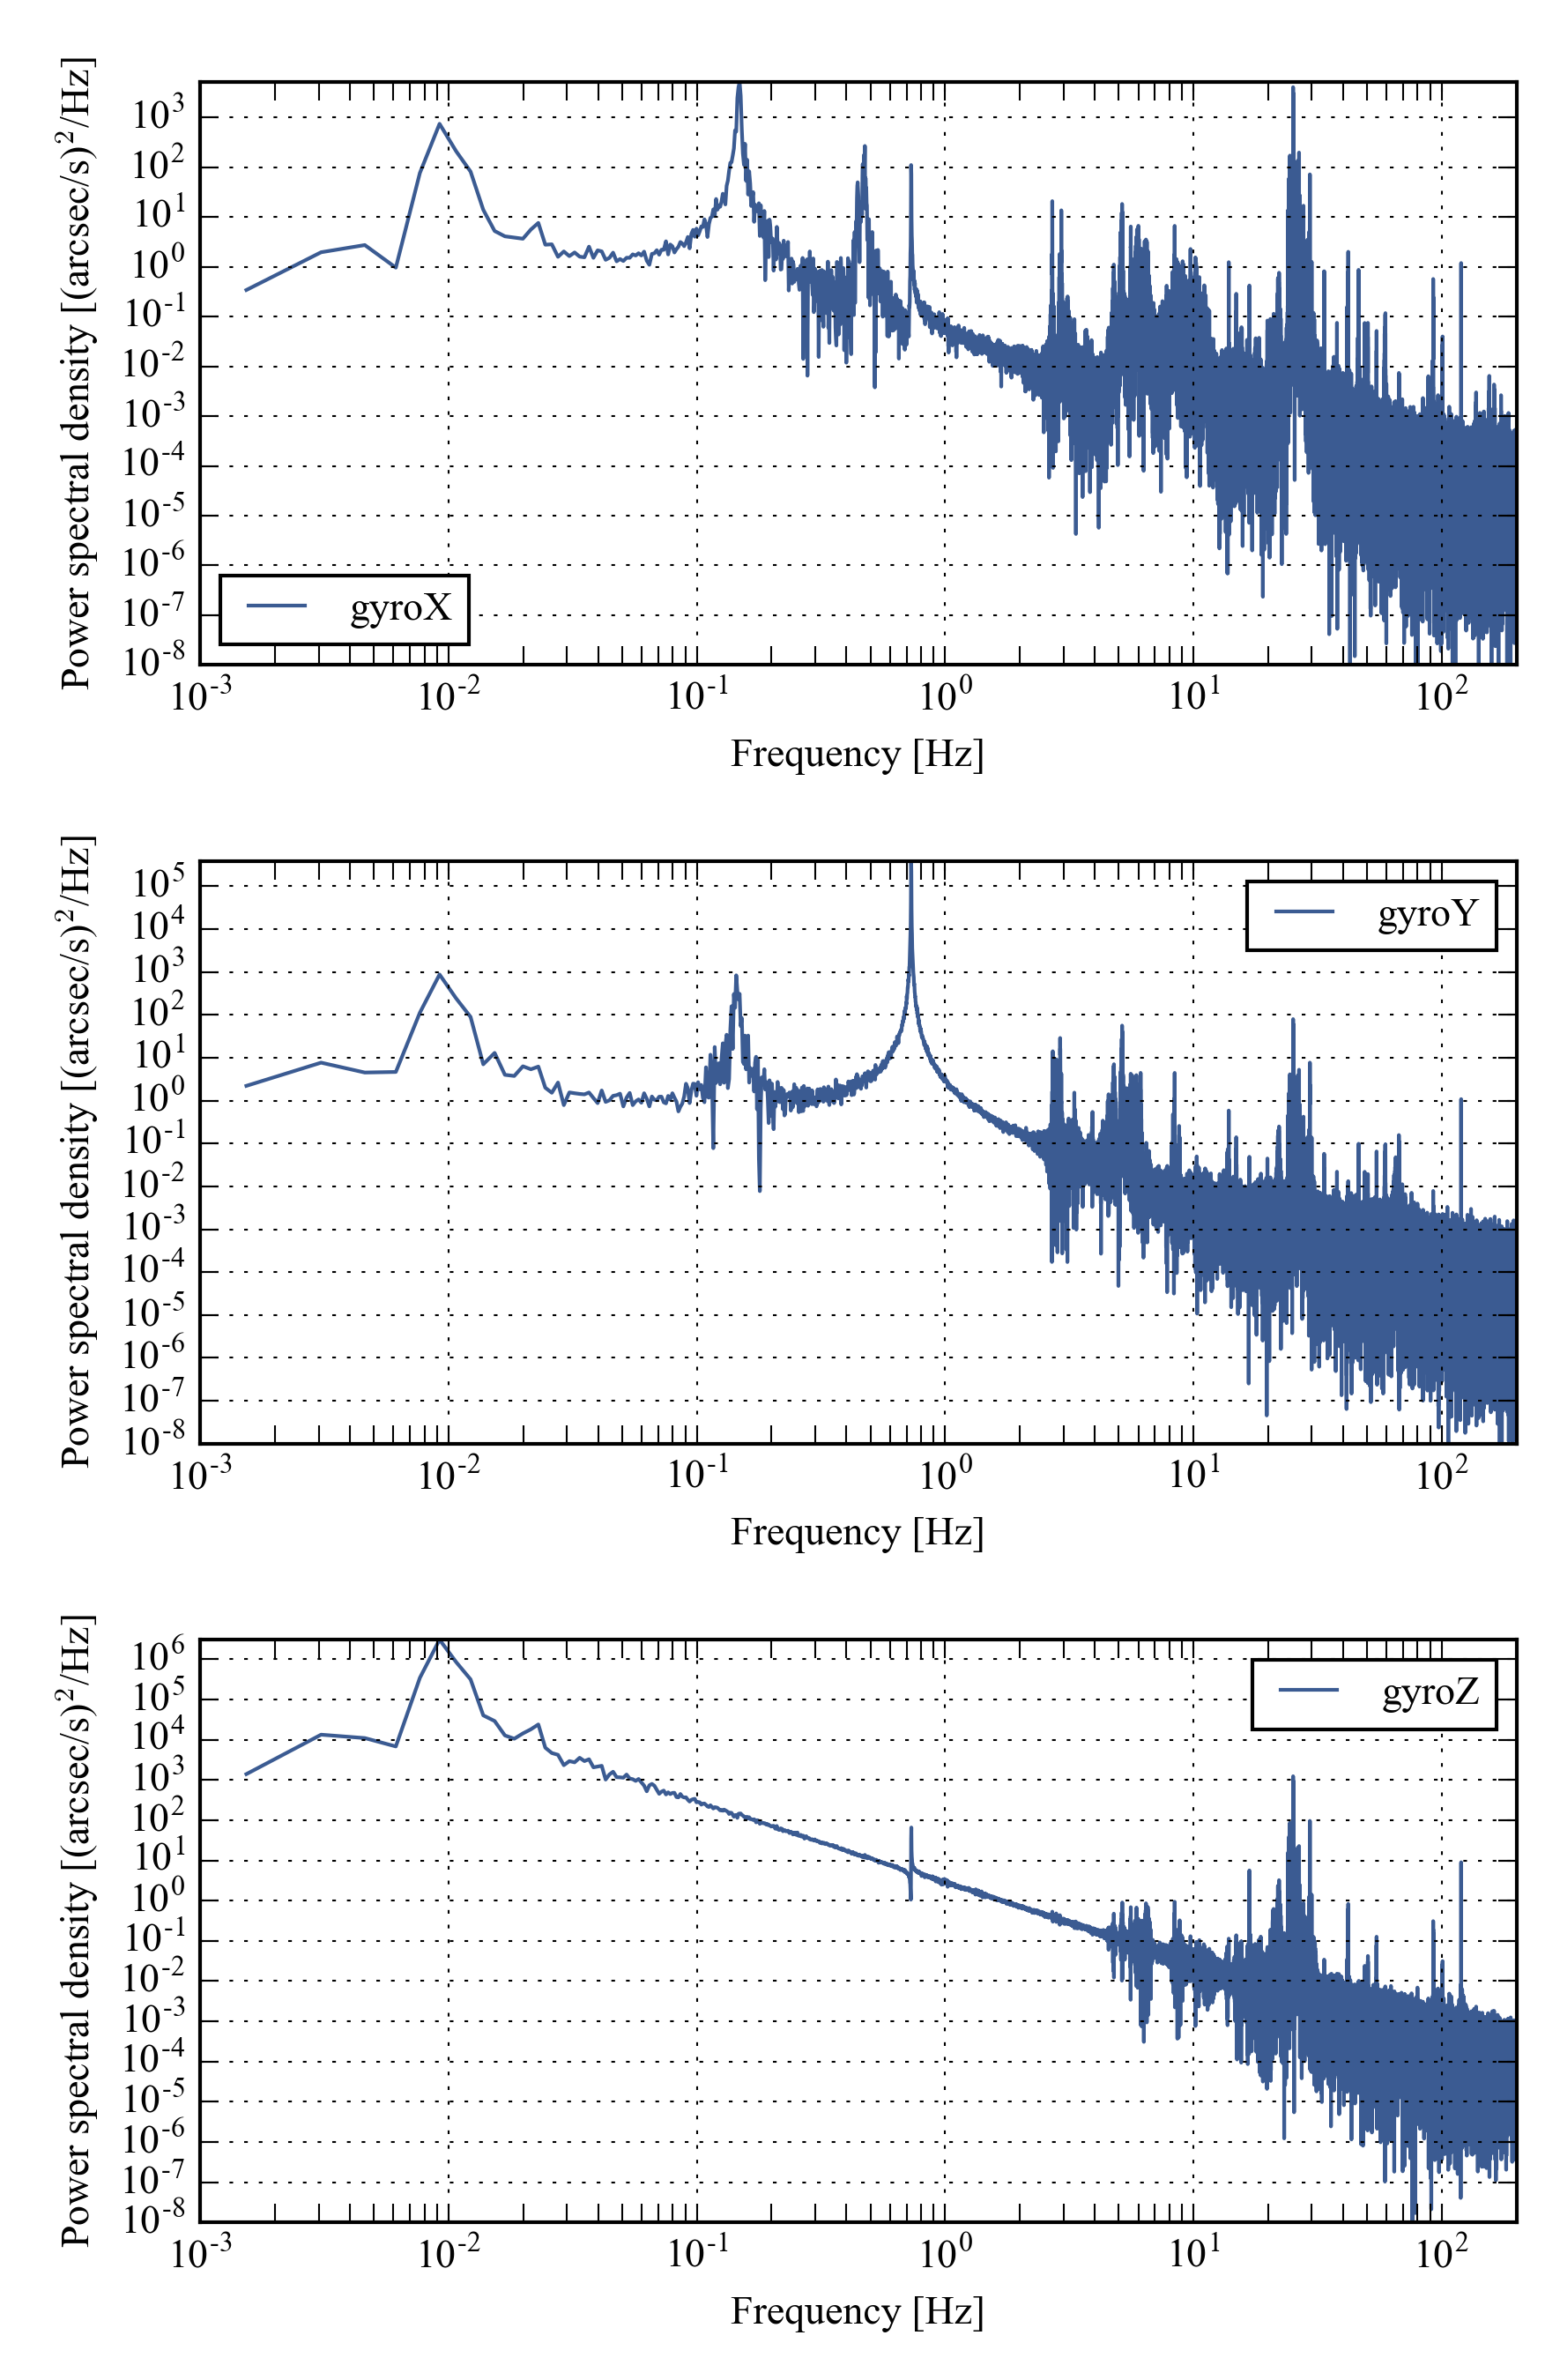
\includegraphics{Figures/lifted_400.png}
\label{fig:multiPSD400_lifted}
\vspace{-0.5cm}
\caption[Gyro PSD with payload lifted]{Gyro PSD with payload lifted.}
\end{center}
\end{figure}


\begin{figure}[!h]
\begin{center}
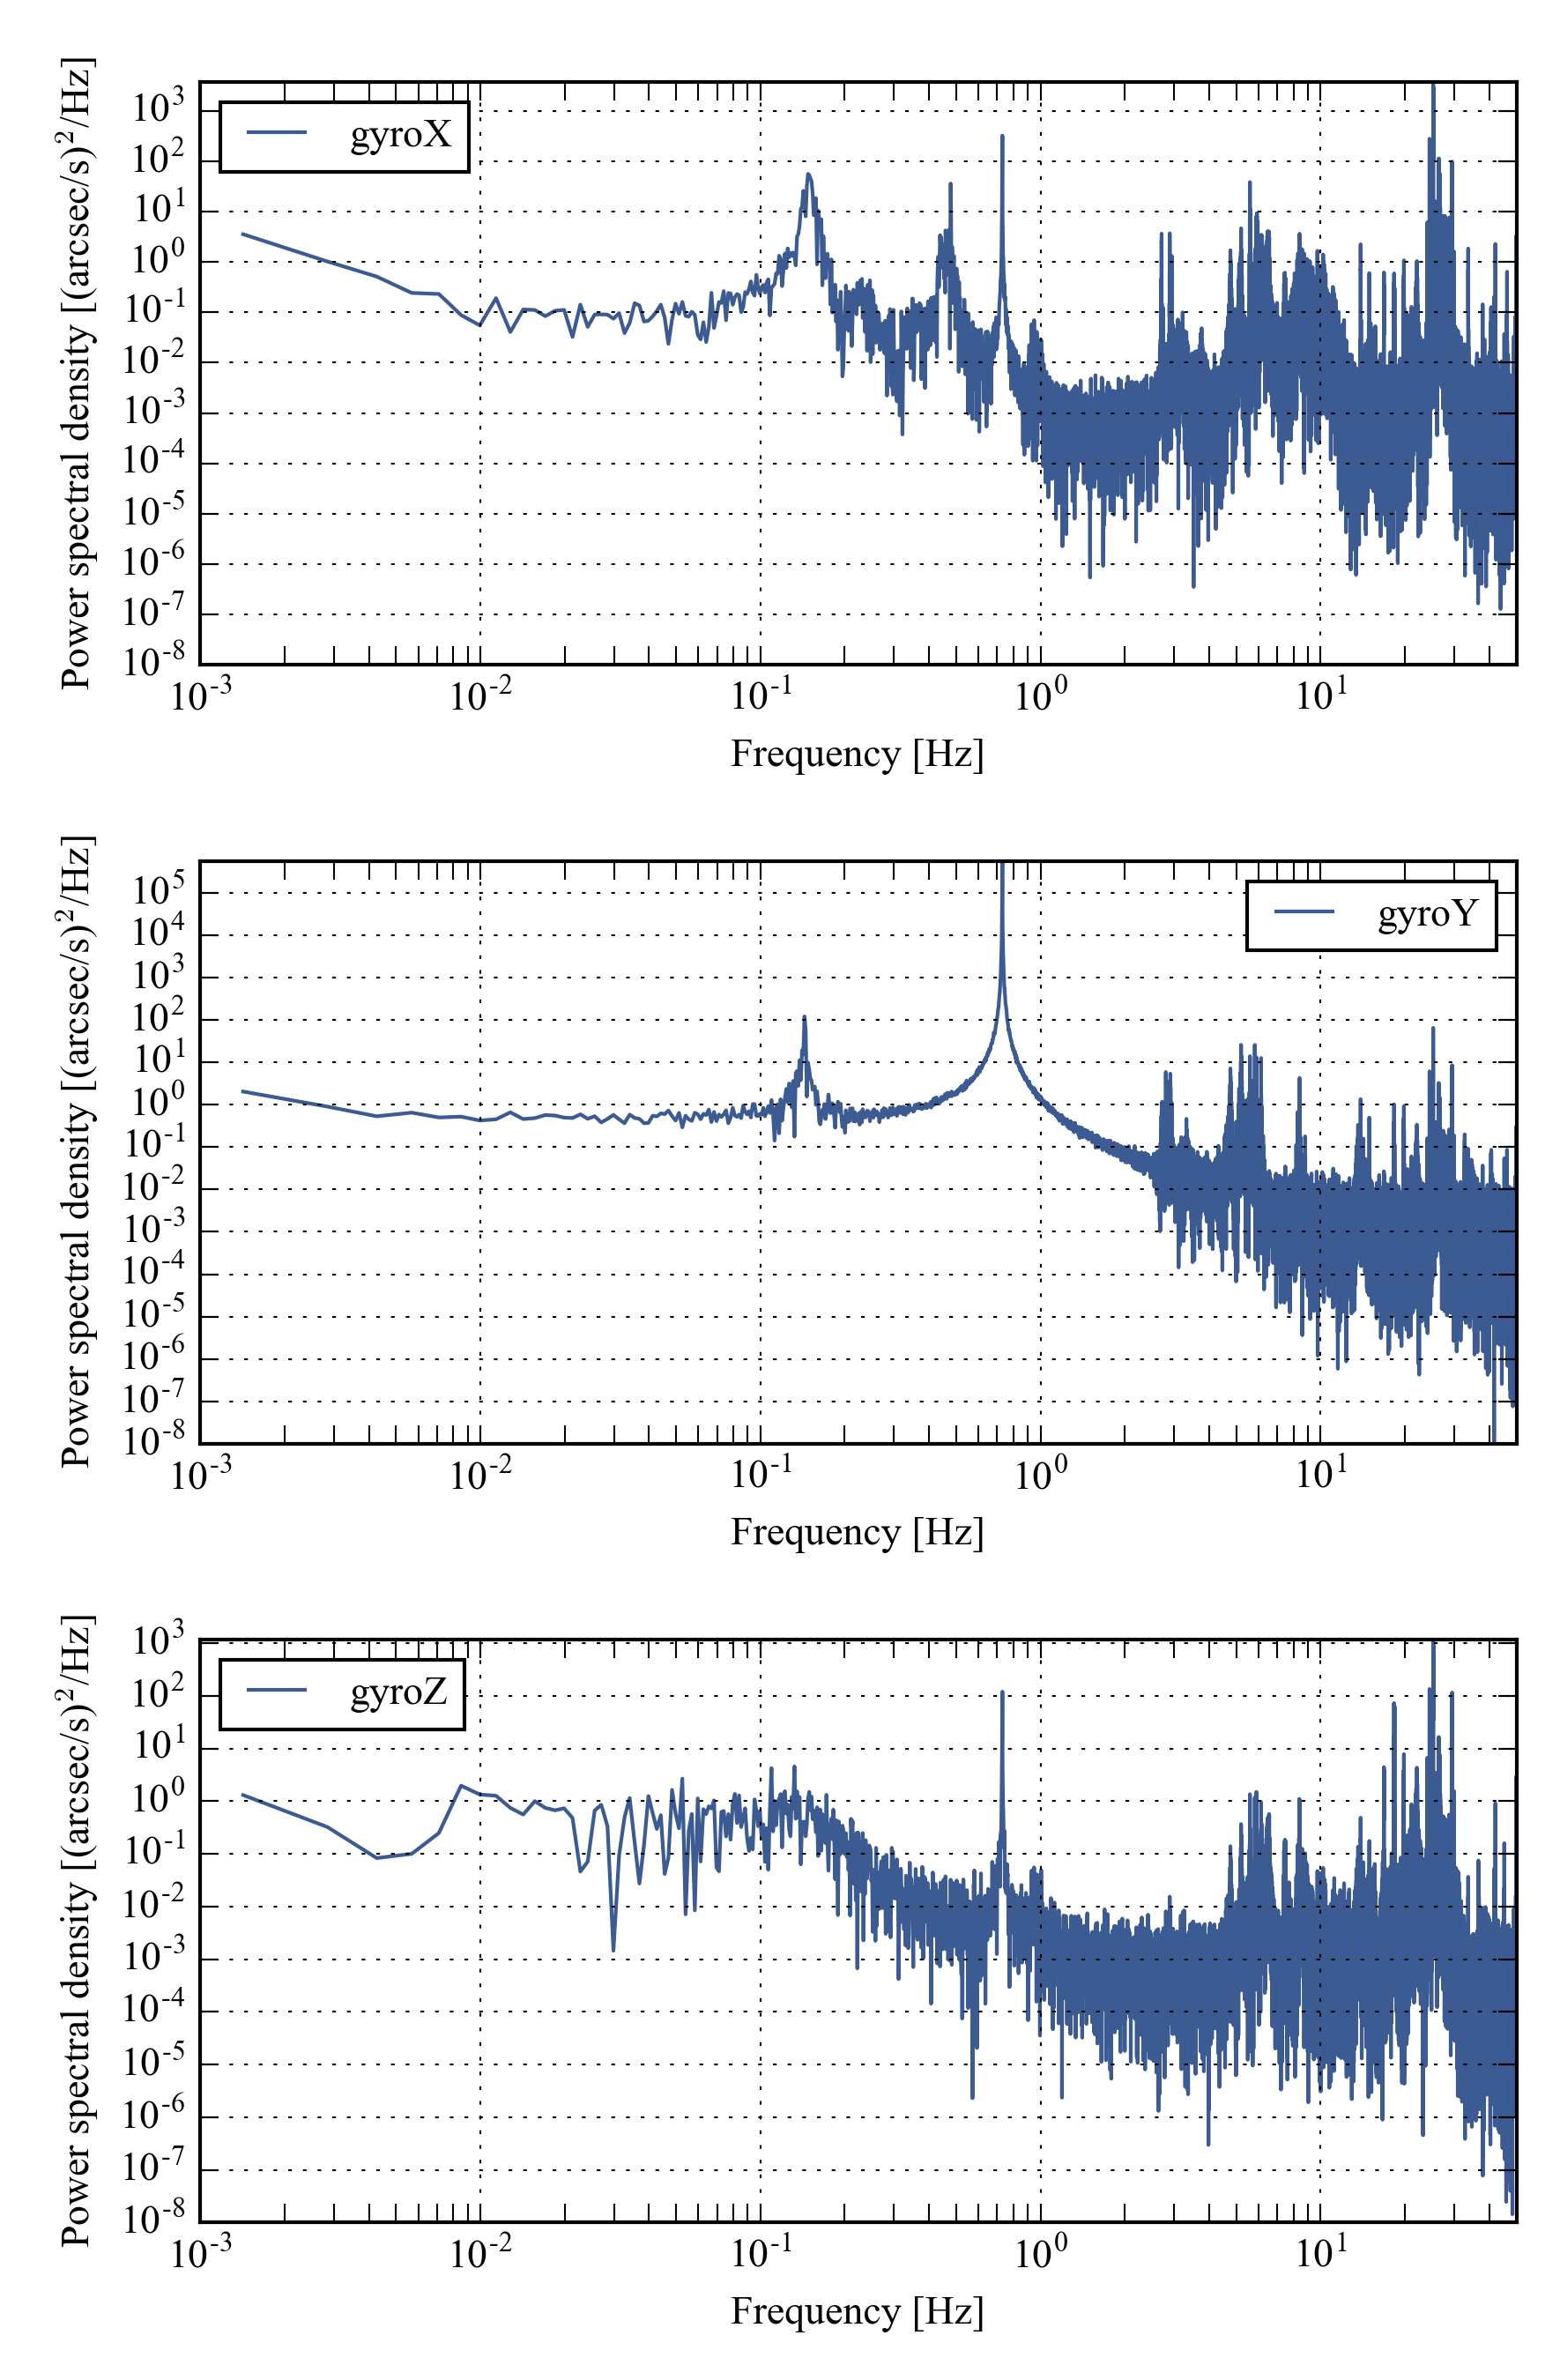
\includegraphics{Figures/multiPSD100.png}
\label{fig:multiPSD100_controlled}
\vspace{-0.5cm}
\caption[Gyro PSD with payload lifted, under azimuth control]{Gyro PSD with payload under azimuth control.}
\end{center}
\end{figure}


 show azimuth stability data
show telescope rolling rms
\subsubsection{With the door open}
\subsection{Kalman filter performance}
Show data with the door open with the star camera acquiring frames
\subsection{gyro+star camera+tip/tilts with CCD cameras}
\subsection{gyro+star camera with H1RG;}

\section{	Using the test results to estimate the flight performance (have to think more about that section)}
\subsection{Perturbation rejection estimates}
\subsection{Pointing knowledge predictions}
\subsection{Pointing control predictions}
